\subsection{Show Content}
\label{sec:configure_show_content}
\label{sec:configure_meta_vars}

This dialog displays all meta variables and DBContent variables for inspection. Previously titled 'Meta Variables', it has been renamed to reflect that it covers the full DBContent schema rather than only the grouped meta variables. \\\\

\begin{figure}[H]
  \centering
  \hspace*{-1cm}
    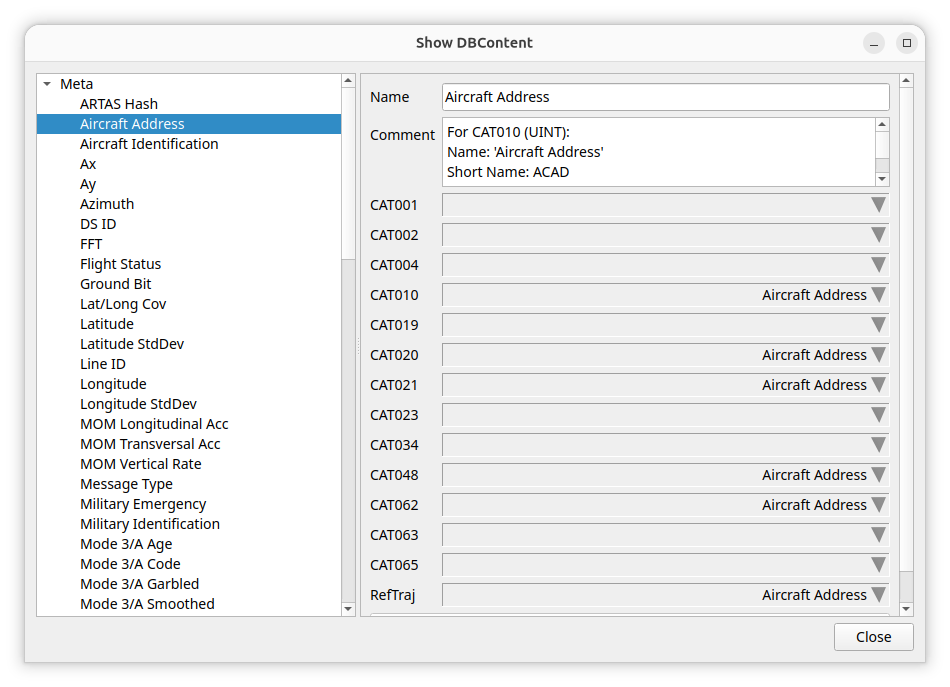
\includegraphics[width=17cm]{figures/configuration_show_content.png}
  \caption{Show Content}
\end{figure}

The content is presented as a flat table with the following columns: \\

\begin{itemize}
\item Name: The variable's name as used inside COMPASS
\item Description: Short description of the variable's meaning
\item Source: Origin or definition of the variable's content
\item Data type: Underlying data type (bool, int, float, string, ...)
\item Unit: Physical unit if applicable
\item Representation: Display representation (decimal, hex, octal, ...)
\item Schema: DBContent the variable belongs to, or empty for meta variables
\end{itemize} \ \\

The 'Source' column reflects what the DBContent definition specifies for each variable. Typical Source values are: \\

\begin{itemize}
\item ASTERIX item references, e.g. 'I020/020.CRT', 'I001/042.X-Component', 'I062/390.CTL.Centre'
\item Calculation hints, e.g. 'Calculated from Time of Day, calendar date', 'Filled by the reconstructor', 'Calculated from Range, Azimuth (radar polar->WGS-84 projection)'
\item Internal hints, e.g. 'Internal: import line/source identifier'
\end{itemize} \ \\

Please \textbf{note} that the above are examples of what the 'Source' field can contain - the complete set of possible values is defined by the underlying DBContent configuration. \\

Editing of the displayed entries is gated to \textbf{expert mode}; by default the dialog is read-only. Expert mode can be enabled in either of the following ways: \\

\begin{itemize}
\item Pass the '--expert\_mode' command-line flag at application startup
\item Set \texttt{"expert\_mode": true} in \texttt{\textasciitilde/.compass/<version>/task.json}
\end{itemize} \ \\

Please \textbf{note} that no GUI menu toggle for expert mode exists - one of the two methods above has to be used.

\begin{figure}[H]
  \centering
    \fbox{\parbox{0.8\textwidth}{\vspace{1.5cm}\centering \textcolor{red}{\textbf{[FIGURE TODO: 'Show Content' dialog with edit controls enabled in expert mode - capture only if visually different from the read-only state]}}\vspace{1.5cm}}}
  \caption{Show Content in expert mode}
\end{figure}
